% Generated by experiments/synthesis/hw_paper_v4_1.py from the hardware records. Do not edit by hand.
\definecolor{hwblue}{RGB}{31,95,168}\definecolor{hworange}{RGB}{194,87,26}
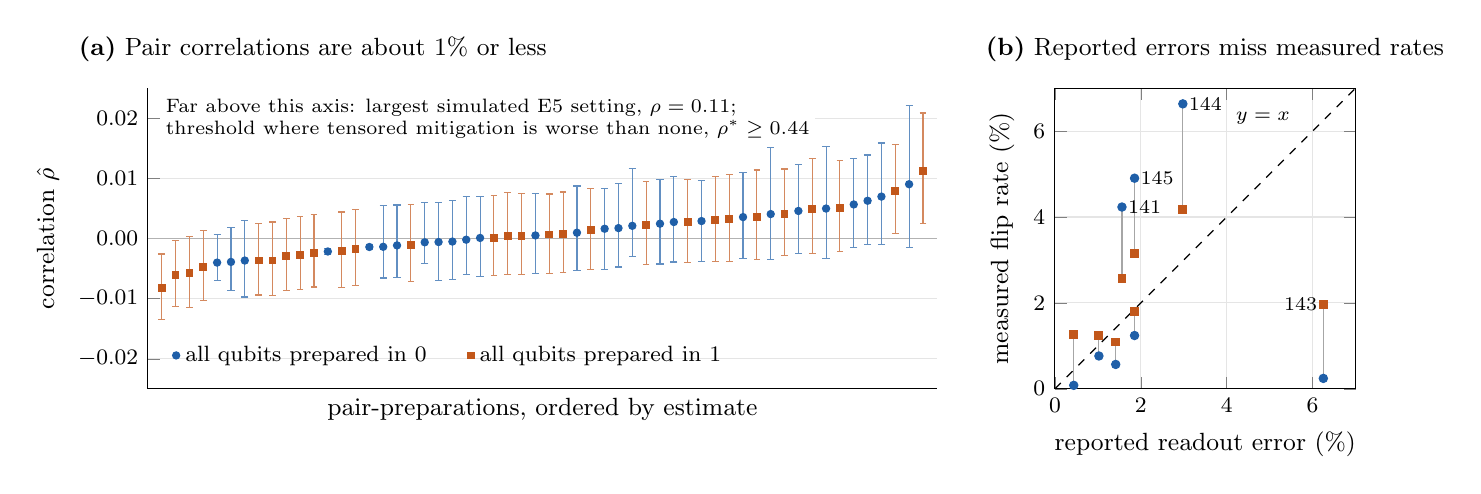
\begin{tikzpicture}
\begin{axis}[name=pa, width=11.6cm, height=5.4cm, xmin=0, xmax=57, ymin=-0.025, ymax=0.025,
  xtick=\empty, ytick={-0.02,-0.01,0,0.01,0.02},
  yticklabel style={/pgf/number format/fixed,/pgf/number format/precision=2,/pgf/number format/fixed zerofill},
  scaled y ticks=false, tick label style={font=\footnotesize}, label style={font=\small},
  xlabel={pair-preparations, ordered by estimate}, ylabel={correlation $\hat\rho$},
  axis lines*=left, ymajorgrids, grid style={gray!20},
  legend style={font=\footnotesize, draw=none, fill=none, at={(0.02,0.04)}, anchor=south west},
  legend columns=2, legend cell align=left, legend style={/tikz/every even column/.append style={column sep=0.45cm}},
  title={\textbf{(a)} Pair correlations are about 1\% or less}, title style={font=\small, at={(0,1)}, anchor=south west, xshift=-1.0cm}]
\addplot[gray!60, forget plot] coordinates {(0,0) (57,0)};
\addplot[only marks, mark=*, mark size=1.3pt, hwblue, error bars/.cd, y dir=both, y explicit, error bar style={hwblue!70}]
  table[x index=0, y index=1, y error plus index=2, y error minus index=3] {
    5 -0.004004 0.004686 0.002994
    6 -0.003896 0.005675 0.004686
    7 -0.003660 0.006582 0.006063
    13 -0.002157 0.000516 0.000556
    16 -0.001409 0.000353 0.000395
    17 -0.001378 0.006882 0.005193
    18 -0.001149 0.006719 0.005374
    20 -0.000631 0.006569 0.003561
    21 -0.000582 0.006588 0.006471
    22 -0.000507 0.006888 0.006347
    23 -0.000196 0.007216 0.005792
    24 0.000095 0.006939 0.006410
    28 0.000514 0.006949 0.006315
    31 0.000965 0.007769 0.006274
    33 0.001623 0.006695 0.006769
    34 0.001730 0.007412 0.006471
    35 0.002109 0.009531 0.005038
    37 0.002463 0.007312 0.006709
    38 0.002744 0.007566 0.006646
    40 0.002903 0.006778 0.006718
    43 0.003566 0.007373 0.006852
    45 0.004064 0.011004 0.007538
    47 0.004585 0.007783 0.007029
    49 0.004984 0.010254 0.008271
    51 0.005664 0.007667 0.007174
    52 0.006278 0.007614 0.007285
    53 0.006970 0.008915 0.008038
    55 0.009030 0.013081 0.010543
  };
\addlegendentry{all qubits prepared in 0}
\addplot[only marks, mark=square*, mark size=1.2pt, hworange, error bars/.cd, y dir=both, y explicit, error bar style={hworange!70}]
  table[x index=0, y index=1, y error plus index=2, y error minus index=3] {
    1 -0.008228 0.005646 0.005304
    2 -0.006026 0.005639 0.005259
    3 -0.005733 0.006058 0.005708
    4 -0.004739 0.006072 0.005577
    8 -0.003650 0.006131 0.005743
    9 -0.003648 0.006394 0.005867
    10 -0.002953 0.006292 0.005643
    11 -0.002711 0.006345 0.005801
    12 -0.002388 0.006308 0.005672
    14 -0.002076 0.006486 0.006038
    15 -0.001750 0.006551 0.006015
    19 -0.001019 0.006691 0.006070
    25 0.000146 0.006952 0.006297
    26 0.000374 0.007264 0.006302
    27 0.000398 0.007052 0.006416
    29 0.000647 0.006754 0.006476
    30 0.000738 0.007005 0.006437
    32 0.001382 0.006933 0.006577
    36 0.002297 0.007145 0.006667
    39 0.002757 0.007087 0.006808
    41 0.003106 0.007249 0.006858
    42 0.003209 0.007371 0.006967
    44 0.003610 0.007779 0.007109
    46 0.004133 0.007433 0.006972
    48 0.004937 0.008338 0.007392
    50 0.005052 0.007872 0.007243
    54 0.007941 0.007664 0.007175
    56 0.011251 0.009621 0.008686
  };
\addlegendentry{all qubits prepared in 1}
\node[font=\scriptsize, align=left, anchor=north west, fill=white, inner sep=2pt] at (rel axis cs:0.015,0.985)
  {Far above this axis: largest simulated E5 setting, $\rho=0.11$;\\threshold where tensored mitigation is worse than none, $\rho^\ast \ge 0.44$};
\end{axis}
\begin{axis}[at={(pa.north east)}, anchor=north west, xshift=1.5cm, width=5.4cm, height=5.4cm,
  xmin=0, xmax=7, ymin=0, ymax=7, xtick={0,2,4,6}, ytick={0,2,4,6},
  tick label style={font=\footnotesize}, label style={font=\small},
  xlabel={reported readout error (\%)}, ylabel={measured flip rate (\%)},
  grid=major, grid style={gray!20},
  title={\textbf{(b)} Reported errors miss measured rates}, title style={font=\small, at={(0,1)}, anchor=south west, xshift=-1.0cm}]
\addplot[black, dashed, forget plot] coordinates {(0,0) (7,7)};
\node[font=\scriptsize, anchor=east] at (axis cs:5.7,6.3) {$y=x$};
  \draw[gray!70] (axis cs:0.439,0.081) -- (axis cs:0.439,1.263);
  \draw[gray!70] (axis cs:1.562,4.233) -- (axis cs:1.562,2.569);
  \draw[gray!70] (axis cs:1.855,1.241) -- (axis cs:1.855,1.799);
  \draw[gray!70] (axis cs:6.250,0.243) -- (axis cs:6.250,1.968);
  \draw[gray!70] (axis cs:1.416,0.568) -- (axis cs:1.416,1.091);
  \draw[gray!70] (axis cs:2.979,6.635) -- (axis cs:2.979,4.181);
  \draw[gray!70] (axis cs:1.855,4.904) -- (axis cs:1.855,3.155);
  \draw[gray!70] (axis cs:1.025,0.765) -- (axis cs:1.025,1.235);
\addplot[only marks, mark=*, mark size=1.5pt, hwblue] coordinates {(0.439,0.081) (1.562,4.233) (1.855,1.241) (6.250,0.243) (1.416,0.568) (2.979,6.635) (1.855,4.904) (1.025,0.765)};
\addplot[only marks, mark=square*, mark size=1.4pt, hworange] coordinates {(0.439,1.263) (1.562,2.569) (1.855,1.799) (6.250,1.968) (1.416,1.091) (2.979,4.181) (1.855,3.155) (1.025,1.235)};
  \node[font=\scriptsize,anchor=west,inner sep=2pt] at (axis cs:1.562,4.233) {141};
  \node[font=\scriptsize,anchor=east,inner sep=2pt] at (axis cs:6.250,1.968) {143};
  \node[font=\scriptsize,anchor=west,inner sep=2pt] at (axis cs:2.979,6.635) {144};
  \node[font=\scriptsize,anchor=west,inner sep=2pt] at (axis cs:1.855,4.904) {145};
\end{axis}
\end{tikzpicture}
